%!TEX root = ../physical-olympics-2.tex
\chapter{量子论}

我们用选自\emph{费曼}(R. Feynman)先生的物理学讲义的开篇金句来作为本章与下一章近代物理内容的开头:
\begin{quote}
Each piece, or part, of the whole of nature is always merely an approximation to the complete truth. Therefore, things must be learned only to be unlearned again or, more likely, to be corrected. The test of all knowledge is \emph{experiment}. Experiment is the sole judge of scientific ``truth''.
\end{quote}

的确,\,量子理论以其不直观而被近代早期物理学家们所疑惑,\,这其中不乏一些赫赫有名的大师.\,直到现在也有很多基础的问题是没有被深刻地理解的:\,电子的本性与内部结构,\,基本粒子的类别与参数,\,对量子非定域性与测量的理解...\,所以在关于可能会造成问题的领域的学习时,\,需要先明白实验上的事实,\,从中理解理论建立的必要性.


\section{黑体辐射}

对于\emph{热辐射}(thermal radiation)的讨论是何时进入物理研究的视野的呢?\,可以肯定的是人类认识到热辐射现象非常的早:\,光芒万丈的太阳,\,烧红的木炭与金属都是典型的热辐射的情形.\,但人们掌握足够的方法去测量它则也是要到19世纪后半期了.\,热辐射势必涉及到电磁场与电荷的相互作用.\,而且深入到原子尺度,\,实际上就是电磁波的发射与吸收.\,对于电磁波的发射,\,我们在电磁学中粗略讲过,\,只要有加速运动的电荷就会导致电磁辐射.\,之后小节我们将认识到微观电荷不能用``加速''来描述,\,其状态其实是量子态,\,处于激发态才会自发向基态去跃迁放出电磁辐射.\,而对于电磁波的吸收,\,则在光学中我们简要介绍过洛伦兹电子论中的处理方法.\,

\begin{wrapfigure}[9]{o}[0pt]{7cm}
\centering
\vspace{-15pt}
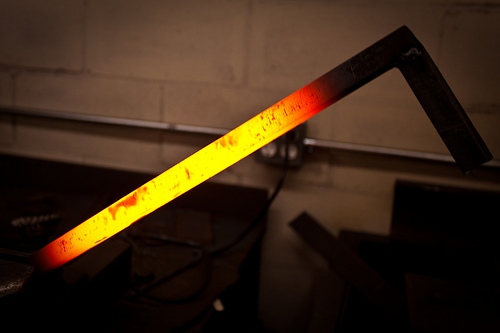
\includegraphics[width=7cm]{image/19-1-1.jpg}
\caption{热辐射}
\end{wrapfigure}
一个物体如果能够在任何温度下把照射到它上面的任何频率的光都全部吸收掉,\,那么这个物体就叫做\emph{黑体}(black body).\,虽然在现实生活中这样的物体并不存在,\,但石墨和碳黑往往被视作比较理想的黑体,\,尽管这样,\,黑体``看上去''也不总是``黑的''.\,著名生物学家查尔斯·达尔文的一个亲戚,\,陶瓷师,\,托马斯·玮致活在1792年注意到所有物体,\,不论化学构成,\,形状,\,尺寸,\,几乎都在相同的温度下烧红.\,黑体也不例外.\,作为这个实验现象研究的推广,\,1859年\emph{基尔霍夫}(G. Kirchhoff)利用热力学理论证明了著名的\emph{基尔霍夫定律}:\,即对于某角频率的光波,\,某温度下任意物体的辐射本领正比于吸收率:
\[e(\omega)=J(\omega,\,T)A(\omega)\]

其中,\,$e$为单位面积单位时间单位角频率间隔辐射的能量,\,而$A$为对该频率光的吸收率.\,$0<A<1$.\,除了吸收以外就是反射.\,物体较薄时还存在透射.\,不同物体在相同的$T,\,\omega$下可以有不同的$A,\,e$,\,但是其比值$J$却是一个\emph{普适}(universal)的函数.\,即与物体本身没有关系.\,而黑体的定义为$A(\omega)$恒等于$1$.\,也就是说明了黑体的辐射本领:
\[e(\omega)=J(\omega,\,T)\]

之后人们的任务就非常清晰了:\,测出不同$T$下的函数$J(\omega,\,T)$.\,而这个过程大致可以分为三个阶段:

1.\,挖掘出$J(\omega,\,T)$的整体特征.

2.\,实验测量$J(\omega,\,T)$的曲线与提出可能的理论模型.

3.\,最终确定$J(\omega,\,T)$的函数形式与理论解释.

\[J(\omega,\,T)=\frac{1}{4}u(\omega,\,T)c\]

\[u(\omega,\,T)=\frac{C_1\omega^3}{e^{C_2\omega/kT}-1}\]

\begin{wrapfigure}[9]{o}[0pt]{7cm}
\centering
\vspace{-15pt}
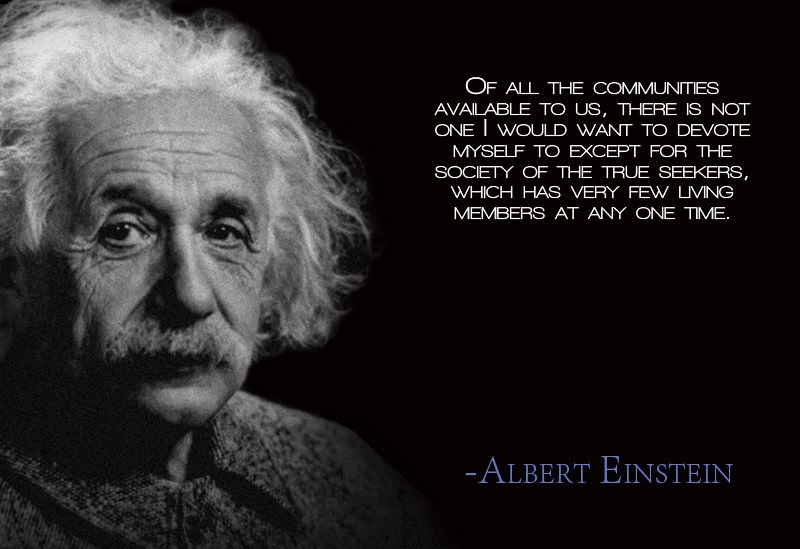
\includegraphics[width=7cm]{image/19-1-2.jpg}
\caption{真正的研究者}
\end{wrapfigure}
怎么去解释这个式子呢?\,从接触到黑体辐射谱的曲线开始,\,普朗克用了足足六年的时间才得到一个合理的解释.\,那是在1901年,\,功夫不负有心人,\,这位``真正的研究者''十分谨慎地发表了关于能量量子化的著名论文,\,科学研究史首次叩响了量子理论的大门.

普朗克的工作大致可以如此解释.\,我们


\begin{itemize}
\item 黑体辐射的性质:
\begin{itemize}
\item 总辐射强度:
\[J=\sigma T^4=\frac{1}{4}uc\]
\[\sigma=5.67\times 10^-8{\rm W/(m^2\cdot K^4)}=\frac{2\pi^5 k^4}{15h^3c^2}\]

\item 辐射频域谱:\,普朗克公式:
\[J(\omega)=\frac{\hbar\omega^3}{4\pi^3c^2}\frac{1}{e^{\frac{\hbar\omega}{kT}}-1}\]

\item 辐射空间谱:\,郎伯定律:
\[\frac{\ud J}{\ud\Omega}=\frac{J}{\pi}\cos\theta\]
\end{itemize}

\item 非黑体满足基尔霍夫定律:\,某角频率$\omega$下发射率$e(\omega)$与吸收率$a(\omega)$必然相等.\,发射率是
\[\frac{\ud E}{\ud S\ud t}=\int E(\omega)\ud \omega\]
\[e(\omega)=E(\omega)/J(\omega)\]

故基尔霍夫定律发现:
\[e(\omega)=a(\omega)\]
\end{itemize}

\section{光粒子性}

\begin{itemize}
\item 光子概念:
\[E=\hbar\omega \quad ,\quad \bs{p}=\hbar \bs{k}\]

\item 用于解释普朗克公式:\,玻色-爱因斯坦统计.

\item 用于解释光电效应:
\[E_k=h\nu-W\geq eU\quad \rightarrow I\]
\end{itemize}

\section{玻尔原子}

\begin{itemize}
\item \emph{精细结构常数}(fine structure constant):
\[\alpha =\frac{e^2}{4\pi \varepsilon_0 \hbar c}\approx \frac{1}{137}\]

\item 半经典假设:\,忽略电子的波动性,\,认为仍然有轨道运动,\,且为圆周运动,\,符合牛顿力学:
\[m\frac{v_n^2}{r_n}=\frac{e^2
}{4\pi \varepsilon_0 r_n^2}\]

\item 量子化假设:\,角动量是量子化的,\,或者作用量量子化:
\[mv_n\cdot 2\pi r_n=nh\]

\item 定态跃迁假设:\,基态$n=1$是能量最低的稳定态,\,其他态与基态彼此之间都有可能发生转变,\,转变是瞬间发生的,\,伴随着一个光子的吸收或发射,\,且需要能量守恒:
\[E_n=\frac{1}{2}mv_n^2-\frac{e^2}{4\pi\varepsilon_0 r_n}\]
\[h\nu=E_n-E_m\]

\item 玻尔理论的解:
\[r_n=n^2 a_0\]
\[v_n=\frac{\alpha c}{n}\]
\[E_n=-\frac{E_0}{n^2}=-\frac{\alpha^2 mc^2}{2n^2}\]

其中$E_0$为第一电离能,\,氢原子为$13.6{\rm eV}$.\,而$a_0$为玻尔半径,\,它与另外两个特征长度:\,电子康普顿波长:
\[\lambda_e=\frac{h}{mc}\]

经典电子半径:
\[r_e=\frac{e^2}{4\pi\varepsilon_0 mc^2}\]

符合;
\[\alpha=\frac{\lambda_e/2\pi}{a_0}=\frac{a_0}{r_e}\]

\end{itemize}

%\section{电子波动性}

\section{物质波与波函数}

\begin{itemize}
\item 匀速运动的粒子对应一个平面波;
\[\psi=Ae^{\ui(\omega t-\bs{k}\cdot \bs{r})}\]

且符合德布罗意关系:
\[E=\hbar\omega\]
\[\bs{p}=\hbar\bs{k}\]

\item 对这个波的诠释:\,模方表示粒子在某空间点被探测到的概率分布函数:
\[f(\bs{r})=|\psi|^2\]
\[\int f(\bs{r})\ud V=1\]

\item 测不准原理:\,平面波情况下粒子位置是不确定的,\,但是动量却唯一.\,任意一个波函数可以分解为不同概率的平面波的叠加,\,那么某方向上位置和动量的两个不确定度(标准差)满足:
\[\Delta x\Delta p\geq \frac{\hbar}{2}\]

\end{itemize}
